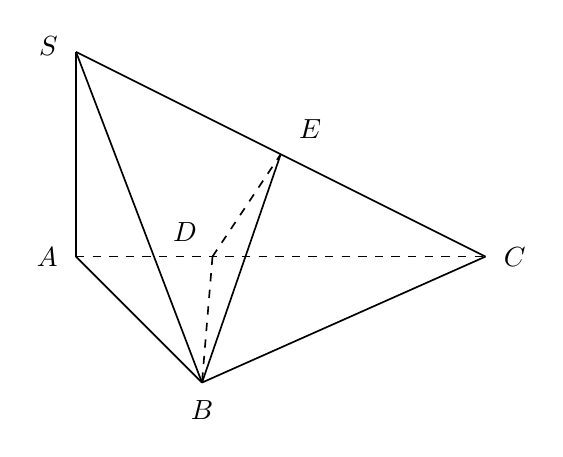
\begin{tikzpicture}[x=1cm,y=1cm,line width=.6pt]
% Triangular pyramid S-ABC, SA vertical, E on SC, D on AC.
\coordinate (S) at (0,4.2);
\coordinate (A) at (0,1.6);
\coordinate (B) at (1.6,0);
\coordinate (C) at (5.2,1.6);
\coordinate (E) at (2.6,2.9);
\coordinate (D) at (1.733333333,1.6);
% base + lateral
\draw (S) -- (A);
\draw (S) -- (B);
\draw (S) -- (C);
\draw (A) -- (B);
\draw (B) -- (C);
\draw[dashed] (A) -- (C);
% interior segments
\draw (B) -- (E);
\draw[dashed] (D) -- (E);
\draw[dashed] (D) -- (B);
% labels offset clear of strokes
\node[left,xshift=-3pt,yshift=2pt] at (S) {$S$};
\node[left,xshift=-3pt] at (A) {$A$};
\node[below,yshift=-3pt] at (B) {$B$};
\node[right,xshift=3pt] at (C) {$C$};
\node[above right,xshift=3pt,yshift=2pt] at (E) {$E$};
\node[above left,xshift=-2pt,yshift=2pt] at (D) {$D$};
\end{tikzpicture}
